\section{Experimental Results}

\subsection{Tuning System Gains}
\begin{frame}{\thesection. \insertsection \ - \insertsubsection}
	Tuning the Kalman Filter gains is difficult and time consuming!
	\begin{enumerate}
		\item Gather baseline data for the \textbf{mobile phone}. Run and walk in a straight line,
		circle, square, etc.
		\item Tune corresponding noise parameters for IMU and GPS position, speed and velocity data
		until the extimated trajectory is accurate.
	\end{enumerate}
\end{frame}

% ----------------------------------------------------------------------

\begin{frame}{\thesection. \insertsection \ - \insertsubsection}
	\begin{enumerate}
		\setcounter{enumi}{2}
		\item Gather baseline flight data: Land on a static mobile phone, follow
		phone and land on a moving phone.
		\item Tune gains relating to the MAV INS and review mobile phone tuning until
		the data reflects the flight test.
	\end{enumerate}
	No vision sensors yet!
\end{frame}

% ----------------------------------------------------------------------

\begin{frame}{\thesection. \insertsection \ - \insertsubsection}
	\begin{enumerate}
		\setcounter{enumi}{4}
		\item Tune the gains for the vision sensors i.e. AprilTag detection by the gimbaled and fixed cameras.\\
		We used a motion capture system to compare ground truth data and the filter's output.
		\item \textbf{Final step} : Tune the filter as a whole on full landing tests and make sure 
		there are no regressions on the baseline data. The goal is to tune the relative weights of all
		sensors w.r.t each other.
		
	\end{enumerate}
\end{frame}

% ----------------------------------------------------------------------

\begin{frame}{\thesection. \insertsection \ - \insertsubsection}
	Tuning the \textbf{Controller Gains} is easier than the estimator gains.
	\begin{itemize}
		\item We use DJI's proprietary simulator to simulate the approach and landing phases in order to tune
		the PN controller, the switching distance and the PD controller.
		\item Flight tests allow validation and testing under windy conditions.
	\end{itemize}
\end{frame}

% ----------------------------------------------------------------------


\begin{frame}{\thesection. \insertsection}
	\begin{figure}
		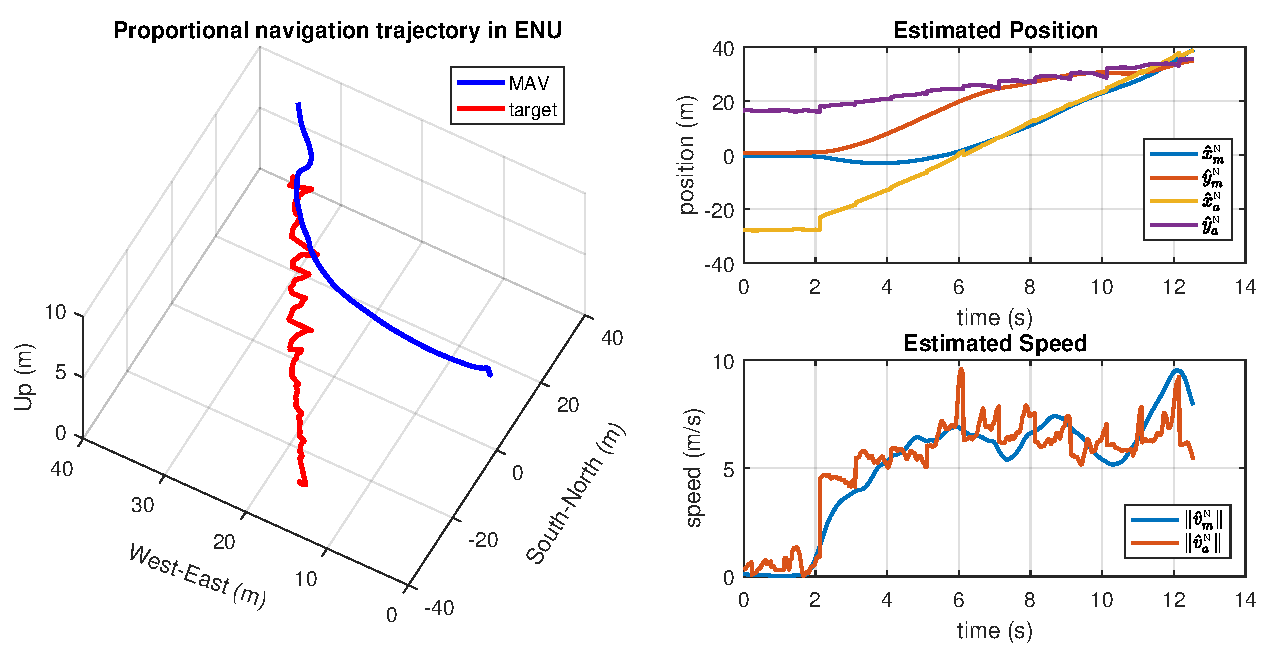
\includegraphics[width=0.8\paperwidth]{figures/pn.pdf}
		\caption{Straight line trajectory test of the PN controller.}
	\end{figure}
\end{frame}

% ----------------------------------------------------------------------

\begin{frame}{\thesection. \insertsection}
	\begin{figure}
		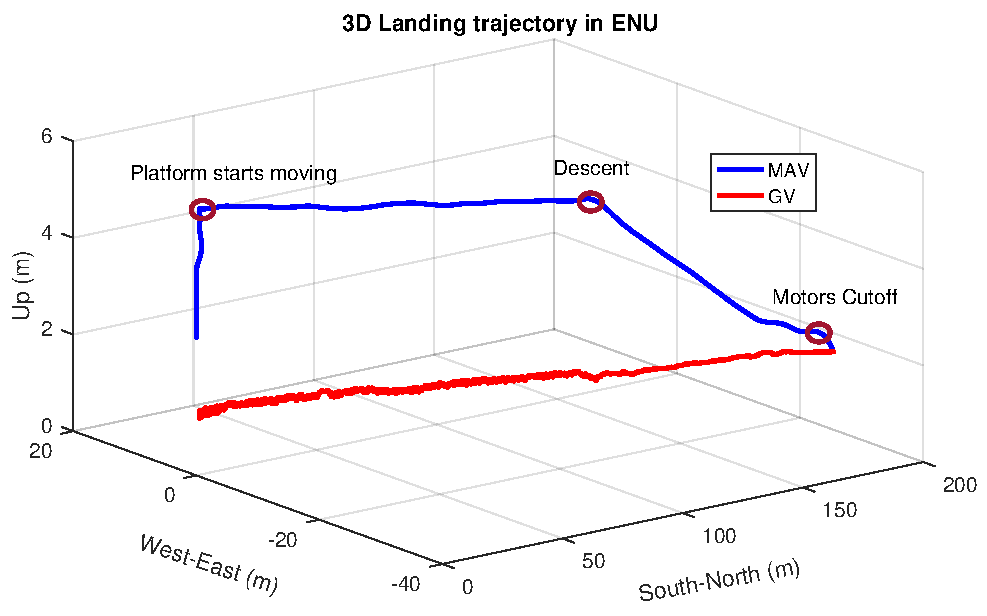
\includegraphics[width=0.8\paperwidth]{figures/landing.pdf}
		\caption{Side view of the MAV landing on a moving car at 50 km/h with only the close range controller.}
	\end{figure}
\end{frame}

% ----------------------------------------------------------------------

\begin{frame}{\thesection. \insertsection \ - \insertsubsection}
	\begin{figure}
		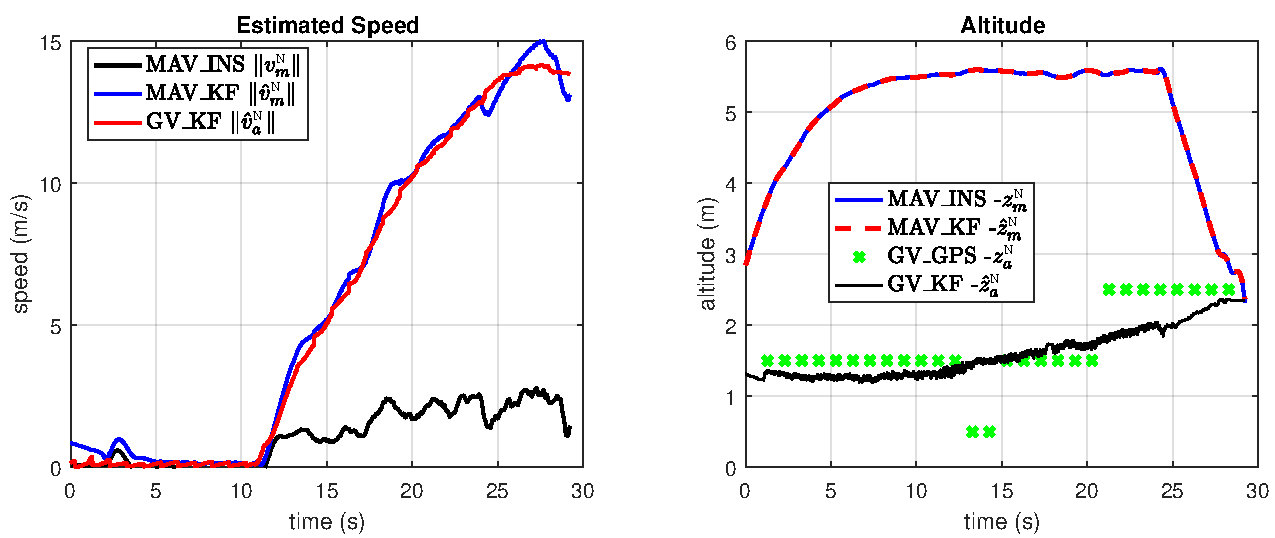
\includegraphics[width=0.8\paperwidth]{figures/landing_motion.pdf}
		\caption{Kalman filter outputs during flight. Notice the INS' velocity output is invalid
		when the MAV is on top of the landing platform.}
	\end{figure}
\end{frame}

% ----------------------------------------------------------------------

\begin{frame}{\thesection. \insertsection}
	See video.
\end{frame}

% ----------------------------------------------------------------------

\begin{frame}{\thesection. \insertsection}	
	Why did it slip at $50$ km/h ?
	\begin{enumerate}
		\item Close to top speed of the MAV 
		\item We introduced a small delay before motor cutoff to allow the MAV to straighten out.
		\item At these speeds, airflow around the car becomes significant.
	\end{enumerate}
	The last two points combined give the MAV just enough lift to slide backwards.
\end{frame}